%% Autor: Björn Ritterbecks 
%% Letzte Aenderung: 15.06.2016 
\thisfloatsetup{%
  capbesidewidth=\marginparwidth}
\begin{figure}[htbp]
\centering
%\sansmath
 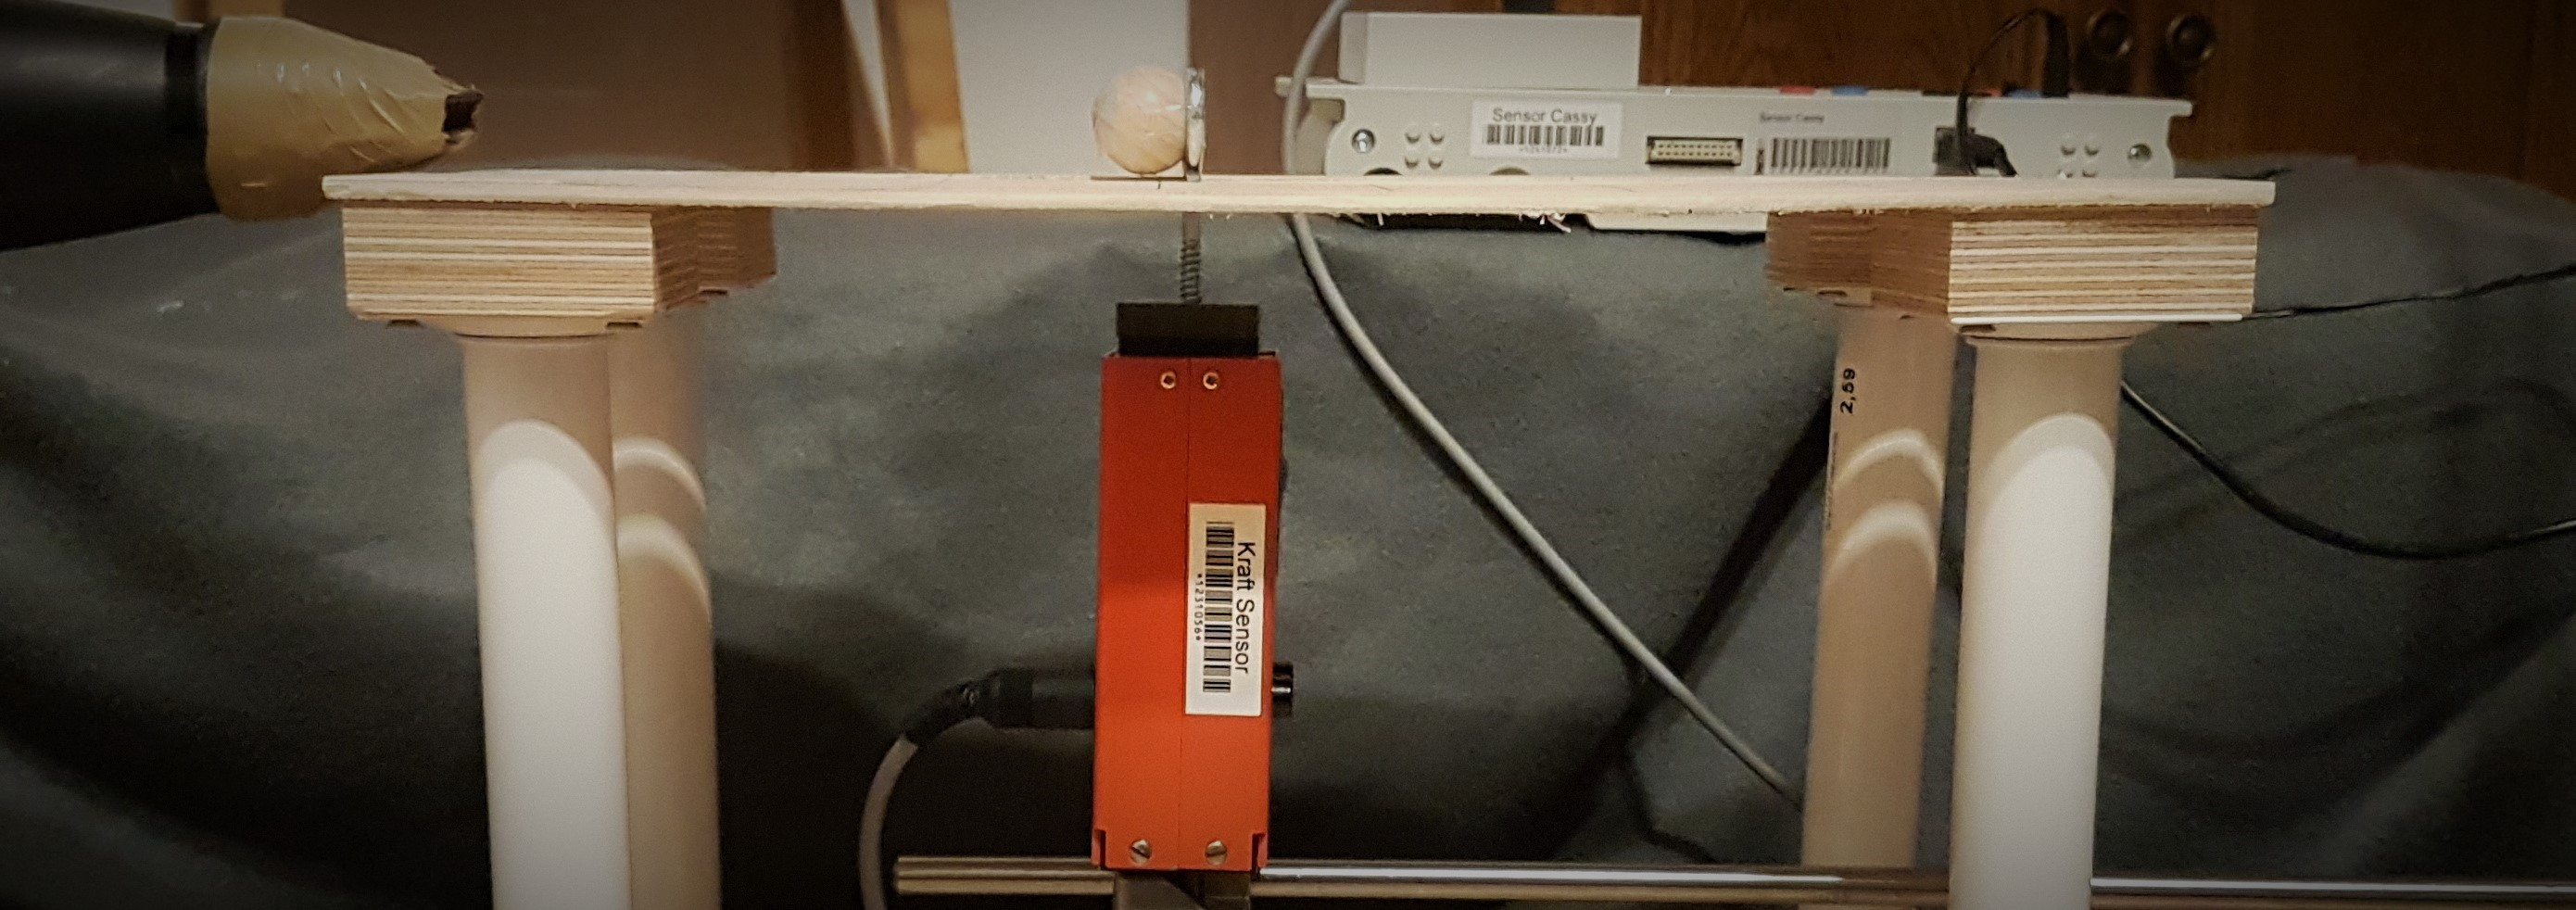
\includegraphics[width=0.99\textwidth]{images/stroemungskraftmessung3.jpg}
  \caption[Coulomb-Kraftmesser der Firma LD Didactic]{Die orange-farbige Box in der Mitte des Fotos vom Messaufbau ist ein Coulomb-Kraftmesser. Dieser ist in $x$-Richtung beweglich an eine Stativstange montiert. Ein eingeschraubter Haken ermöglicht die Befestigung von zu vermessenden Luftwiderständen.}
    \label{fig:stroemungskraftmessung3}
  \vspace{-0pt}
\end{figure}